\section{Framework and overview}\label{sec:framework}

\begin{figure}[h]
\centering
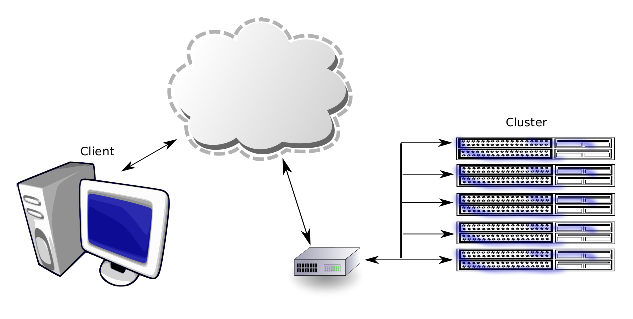
\includegraphics[scale=0.85]{img/framework.eps}
\caption{Testbed setting used for evaluation}
\label{fig:framework}
\end{figure}

\subsection{testbed}
The testbed consists of 5 machine containing a quad-core Xeon 2135, 16GB RAM and commodity 500GB 7.2k rpm disks running stock Ubuntu 12.04. They are interconnected with 1Gbps Ethernet on a single switch. A separate machine acts as client without being a Zookeeper server. The Round-Trip Time~(RTT) between machines in the cluster is around 0.1ms and around 0.2ms for client to cluster communication. For our experiments these nodes for quorums out of 1, 3 or 5 nodes as indicated. The server-side uses Zookeeper version 3.3.5 whereas the client-side implementation of benchmarks uses the respective Python bindings for the baseline "smoke test" and Java bindings for locks and queues implementations.
In order to control the impact of client-server and server-server latency we manually set the transmission latency of packets transmitted between nodes using the Linux "Traffic Control" utility. We automate the process of enumerating client-server and server-server latency pairs and repeatedly run the experiments and average the results to reduce the impact of jitter.

\subsection{consensus protocol}
It is important for distributed systems to have a well-defined consensus protocol. High latency and possibility of failures make achieving consensus an intricate task. For this matter consensus protocols such as Two-Phase Commit~(2PC), Three-Phase Commit~(3PC), and paxos were proposed. In this section we will focus on paxos due its use in distributed consensus services, such as Chubby and, to a large degree degree, Zookeeper. The use of paxos over other alternatives is its resilience to node and network failures. In addition, paxos does not need a fail recovery model.

At each iteration, a \emph{proposer} initiates the protocol and send a proposal to other nodes. Each proposal is tagged with a unique sequence number. Other nodes are called \emph{acceptors}. When acceptors receive proposals, they would either accept or reject. Accepting a proposal is essentially a promise not to accept other proposals with lower sequence numbers. When a majority (quorum) of servers accept a value, then the proposer can proceed with committing the proposal by sending a commit message to all followers. 

\subsection{Zookeeper}
Zookeeper is an open-source coordination service for distributed systems. It runs as a set of replicated distributed servers. A leader election mechanism is used. All requests are forwarded to the leader. A consensus protocol is used to agree on received requests. A combined transaction and write-ahead logging is used in a variant of Paxos as a consensus protocol. Zookeeper levarage an \emph{atomic broadcast} protocol in their consensus protocol implementation. Clients can connect to any of those replicas and issue operations. Zookeeper maintains an order of operations. Each update is stamped. This stamp can then be levaraged in higher level abstractions. Guarantees made by Zookeeper to clients' operations include the following:
\begin{itemize}
\item{\emph{Sequential consistency}: operations are executed in the order they were received. }
\item{\emph{Atomicity}: operations are either completely executed or aborted. }
\item{\emph{Single system image}: all servers maintain the same view. }
\item{\emph{Reliability}: updates are persistent. }
\item{\emph{Timeliness}: updates will be reflected on all servers within a specified time bound. }
\end{itemize}
These guarantees will aid us in reasoning on the way we use Zookeeper operations. The set of offered operations enable more complex services such as coordination, synchronization, configuration management, and naming. These operations operate on a Unix-like filesystem tree architecture. Each file has a path and could be either \emph{permanent} or \emph{ephemeral}. Permenant files persist a client's disconnection whereas ephemeral files are deleted when a client disconnects. Those "files" are called \emph{znodes}. A useful zookeeper primitive is \emph{watch}. A user can set a watch on a znode. When a change on the state of that znode occur, the watch is triggered and the user is informed on the new state of the znode. We now summarize Zookeeper operations of our interest:
\begin{itemize}
\item{\emph{create}: create a znode by specifying a path. A \emph{sequenced} flag can be used to tell Zookeeper to append the znode name with a monotonically increasing identifier. Pathname is returned if create is successful. Otherwise, an exception is returned.}
\item{\emph{delete}: deletes a znode.}
\item{\emph{exists}: checks if a znode exists on a supplied location.}
\item{\emph{getChildren}: return a list of children of a znode, hence files in a folder.}
\end{itemize}
Each one of those operations have two implementations, a synchronous and an asynchronous ones. Synchronous operations block until a reply is received from the server. On the other hand, asynchronous operations returns immediately and a callback is set on the client side to receive from the server when operation is complete.

\begin{figure}[h]
\centering
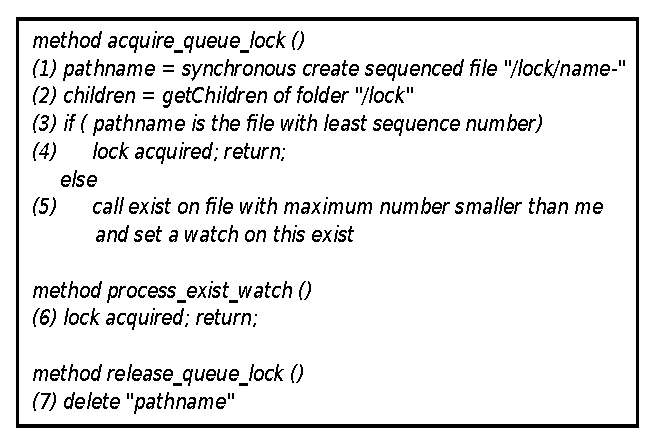
\includegraphics[scale=0.85]{img/queue_lock_pseudo.eps}
\caption{Pseudo code of acquiring and releasing queue locks}
\label{fig:queue_lock_pseudo}
\end{figure}

\begin{figure}[h]
\centering
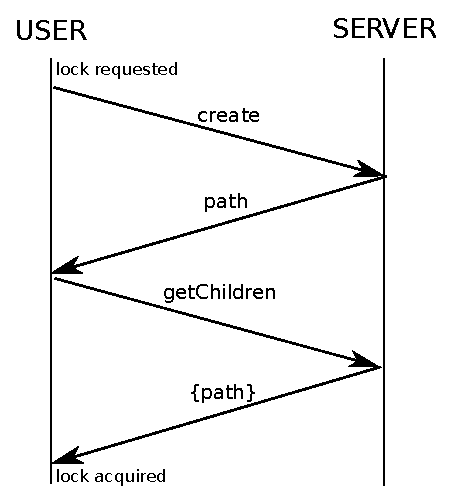
\includegraphics[scale=0.85]{img/queue_lock_time.eps}
\caption{A time diagram showing time required to acquire a queue lock if no other user is holding it}
\label{fig:queue_lock_time}
\end{figure}

\begin{figure}[h]
\centering
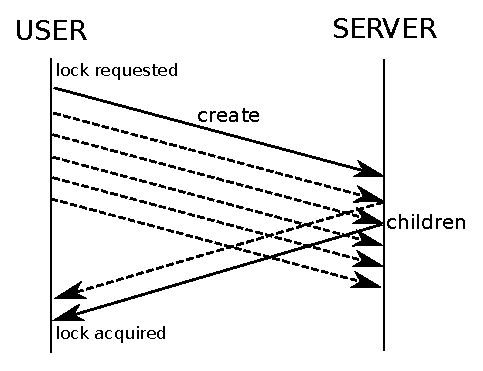
\includegraphics[scale=0.85]{img/async_queue_lock_time.eps}
\caption{A time diagram showing time required to acquire a queue lock if no other user is holding it using asynchronous calls. Dashed arrows from user to server are getChildren operations. Dashed arrows from server to user represent getChildren replies before the lock is acquired. Solid arrow from server to user is getChildren reply with user having the smallest sequenced file. The callback for asynchronous create is not shown.}
\label{fig:async_queue_lock_time}
\end{figure}

\subsection{synchronization primitives}

One of the main points studied in this paper is the effectiveness of synchronization mechanisms (primitives) and their behavior under different network conditions and contention levels. Here, we give a summary of the primitives and implemetations we consider. Primitives are queue locks and test-and-set~(TAS) and implementations are divided into synchronous and asynchronous depending on the pattern of client-server interactions. We translate the primitives into an actual implementation using Zookeeper.

\subsection{Synchronous test-and-set lock}

To acquire a lock, the client repeatedly executes atomic test-and-set (TAS) until it succeeds. TAS typically tests a boolean flag until it flips it from false to true and returns sucessfully. Initially, TAS surfaced in bus-based shared memory systems due to the advent of atomic TAS operations. In Zookeeper we are able to create a primitive that is similar in spirit to hardware TAS. The client tries to create a node with a known name (all competing clients try to create the same node). If the file already exists the create operation fails, which means that another client is holding the lock. On a successful response, the client obtains the lock. To release the lock, the node is deleted. We repeatedly try to acquire a lock by calling \emph{create} in a busy loop. Alternatively, a watch on the file can be used to avoid busy waiting. Apparently, whichever request arrives first after the lock is cleared is served. There is no order as in entering a queue which impacts fairness. The execution path of TAS when no client is holding the lock is only one synchronous \emph{create} call. Otherwise, it is the time until the client happens to be the fastest to re-create the file after deletion.

\subsection{Synchronous queue lock}

This lock uses a queue structure maintaing the process of acquiring a lock. If a client tried to acquire a lock while another was holding it, then the request is queued. Thus, clients acquire the lock based on the order in which they entered the queue, helping achieve fairness. This is implemented in Zookeeper following the "queue recipe" by synchronously creating an ephemeral, sequenced znode. The create operation returns the file name, indicating the sequence number. The client the gets all sibling nodes and determines its predecessor. The client then installs a watch for deletion of this node, i.e. the client waits until it posesses the smallest sequence number. When the watch response returns the lock is considered acquired. Later, the lock is released by merely deleting the previously created node. Pseudo code is displayed in Figure~\ref{fig:queue_lock_pseudo}. There are two possible execution paths. First, a client tries to acquire a lock while no one is holding it. In this case algorithm exist in line (4) after calling only two Zookeeper operations, namely synchronous \emph{create} and \emph{getChildren}. Second, another client is holding the lock when we try to acquire it. In this case the total latency is of operations \emph{creat}, \emph{getChildren}, and \emph{exists}, in addition to waiting time until the \emph{watch} returns to the client.

\subsection{Synchronous test-and-set lock}

The asynchonous lock proactively issues asynchronous create requests on a timer basis until a positive response is recorded. This implementation has multiple requests and responses in transit at a time and effectively polls the availability of the lock without dependence on the rount-trip time. In contrast to the synchronous implementation a negative response does not need to transmitted back before a new request can be issued, which allows the next request to arrive at the server within a predetermined period of time. As a trade-off this puts higher load on the network and the quorum, but reduces the time taken to aquire a lock by avoiding an additional notify-request roundtrip.

\subsection{Asynchronous queue lock}

Above, we showed the serial implementation of our queue primitive using synchronous versions of Zookeeper operations. Thus, we block until we receive a reply from the server. We find, however, that we can parallelize create requests and obtaining the Id of the predecessor to reduce latency. We issue the create request ansynchonously and immediately start polling for its siblings by issuing asynchonous getChildren requests on a timer basis. As soon as the create response returns the Id, the most recent list of siblings containing this Id ("consistent list") can be analyzed to either find the lock acquired or determine the predecessor. This implementation has multiple requests and responses in transit at a time and effectively "polls" the availability of the lock. This puts higher load on the network and multiple read requests on the server, but in the optimal case cuts the time taken to aquire a lock by avoiding the delay for receiving the response to the create request and only then issuing the getChildren request. Further analysis shows that the overhead of polling for longer wait times can be cut off after receiving the consistent list of sibling by installing a watch on the predecessor and as for the synchronous queue.

For illustration the time required to acquire a lock when no user is holding it for a synchronous queue lock is two RTTs as shown in Figure~\ref{fig:queue_lock_time}. However, as shown in Figure~\ref{fig:async_queue_lock_time} we can proceed with calling parallel \emph{getChildren} operations after the asynchronous create. Latency in this case is one RTT plus the time required to create the file and half the latency between \emph{getChildren} requests (remember we are assuming no user held the lock at that time). Likewise, different primitives and asynchronous TAS cut latency in the same way. \note{describe all primitives and put pseudo codes of them if enough time}.
\end{itemize}
